\documentclass[aspectratio=169]{beamer}

\usetheme{Madrid}
\usecolortheme{default}
\usepackage{graphicx}
\usepackage{amsmath}
\usepackage{booktabs}
\usepackage{tikz}
\usetikzlibrary{arrows.meta, positioning, shapes.geometric}

\definecolor{dmblue}{RGB}{66,133,244}
\definecolor{dmgreen}{RGB}{52,168,83}
\definecolor{dmred}{RGB}{234,67,53}

\setbeamercolor{title}{fg=white,bg=dmblue}
\setbeamercolor{frametitle}{fg=white,bg=dmblue}
\setbeamercolor{block title}{fg=white,bg=dmblue}
\setbeamercolor{item}{fg=dmblue}

\title[AlphaStar]{Grandmaster Level in StarCraft II Using\\Multi-Agent Reinforcement Learning}
\subtitle{ECE 752 -- Survey Presentation}
\author{Yehia Fahmy} % TODO: add group members
\institute{University of Waterloo}
\date{Winter 2026}

\begin{document}

% ============================================================
% SLIDE 1: Title
% ============================================================
\begin{frame}
\titlepage
\vfill
\centering
\small Vinyals, Babuschkin, Czarnecki, Silver et al.\ (DeepMind) \\
\textit{Nature}, Vol.\ 575, November 2019
\end{frame}

% ============================================================
% SLIDE 2: Outline
% ============================================================
\begin{frame}{Outline}
\tableofcontents
\end{frame}

% ============================================================
% SECTION 1: Problem & Motivation
% ============================================================
\section{Problem and Motivation}

\begin{frame}{What Problem Does This Work Address?}
\begin{columns}[T]
\column{0.55\textwidth}
\textbf{Goal:} Build an AI agent that plays the full game of StarCraft~II at a professional human level, without simplifying the game.

\vspace{0.5em}
\textbf{Why StarCraft~II?}
\begin{itemize}
    \item Real-time strategy game with $\sim\!10^{26}$ possible actions per step
    \item Imperfect information (fog of war, hidden opponent actions)
    \item Non-transitive strategy space (rock-paper-scissors dynamics)
    \item Long time horizons ($\sim$10 min games, thousands of decisions)
    \item Three asymmetric races: Terran, Protoss, Zerg
\end{itemize}

\column{0.4\textwidth}
\textbf{Game-Theoretic Challenges:}
\begin{itemize}
    \item Cyclic strategies: A beats B, B beats C, C beats A
    \item Na\"ive self-play fails to converge
    \item Must approximate a \textbf{Nash equilibrium} in a complex, non-transitive game
    \item Exploration vs.\ exploitation over vast strategy space
\end{itemize}
\end{columns}
\end{frame}

% ============================================================
% SECTION 2: Prior Work & Limitations
% ============================================================
\section{Prior State-of-the-Art}

\begin{frame}{Prior Approaches and Their Limitations}
\begin{columns}[T]
\column{0.48\textwidth}
\textbf{Previous StarCraft AI agents:}
\begin{itemize}
    \item Simplified the game (restricted maps, units, or rules)
    \item Used hand-crafted sub-systems for micro/macro
    \item Relied on superhuman APM or full map visibility
    \item Rule-based heuristics (search, build-order scripts)
\end{itemize}

\vspace{0.5em}
\textbf{No prior agent} matched overall professional skill in the full, unmodified game.

\column{0.48\textwidth}
\textbf{Related milestones:}
\begin{itemize}
    \item \textbf{Deep Blue} (chess, 1997) -- search-based
    \item \textbf{AlphaGo/Zero} (Go, 2016--17) -- RL + self-play, but perfect information and smaller action space
    \item \textbf{OpenAI Five} (Dota 2, 2019) -- simplified rules, hand-crafted rewards, no camera restriction
\end{itemize}

\vspace{0.5em}
\textbf{Key gap:} General-purpose methods that handle the full complexity of a professional RTS esport.
\end{columns}
\end{frame}

% ============================================================
% SECTION 3: AlphaStar's Approach
% ============================================================
\section{How AlphaStar Advances the Field}

\begin{frame}{Overview of the AlphaStar Approach}
\begin{center}
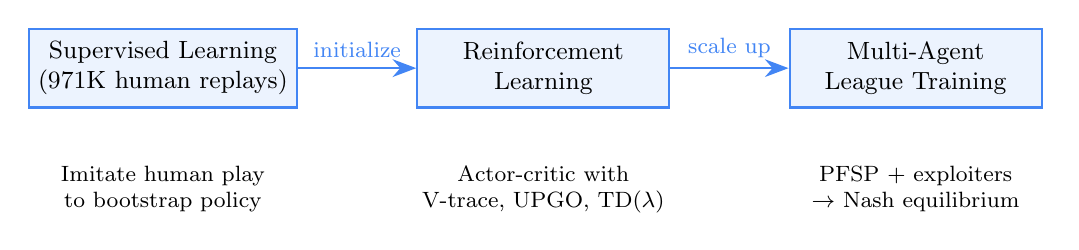
\begin{tikzpicture}[
    box/.style={rectangle, draw=dmblue, fill=dmblue!10, thick,
                minimum width=3.2cm, minimum height=1cm, align=center,
                font=\small},
    arr/.style={-{Stealth[length=3mm]}, thick, dmblue}
]
\node[box] (SL) {Supervised Learning\\(971K human replays)};
\node[box, right=1.5cm of SL] (RL) {Reinforcement\\Learning};
\node[box, right=1.5cm of RL] (League) {Multi-Agent\\League Training};

\draw[arr] (SL) -- node[above, font=\footnotesize]{initialize} (RL);
\draw[arr] (RL) -- node[above, font=\footnotesize]{scale up} (League);

\node[below=0.6cm of SL, font=\footnotesize, align=center, text width=3.2cm]
    {Imitate human play\\to bootstrap policy};
\node[below=0.6cm of RL, font=\footnotesize, align=center, text width=3.2cm]
    {Actor-critic with\\V-trace, UPGO, TD($\lambda$)};
\node[below=0.6cm of League, font=\footnotesize, align=center, text width=3.2cm]
    {PFSP + exploiters\\$\to$ Nash equilibrium};
\end{tikzpicture}
\end{center}

\vspace{0.5em}
\textbf{Key insight:} Combine imitation learning from human data with multi-agent RL in a league of diverse, co-evolving agents to overcome non-transitivity.
\end{frame}

% ============================================================
% SECTION 4: Key Artifacts
% ============================================================
\section{Key Artifacts: Architecture, RL, and League}

\begin{frame}{Neural Network Architecture}
\begin{columns}[T]
\column{0.55\textwidth}
\textbf{Input processing:}
\begin{itemize}
    \item \textbf{Scalar encoder} (MLP): game statistics
    \item \textbf{Entity encoder} (Transformer): per-unit features with self-attention
    \item \textbf{Spatial encoder} (ResNet): minimap features
\end{itemize}

\vspace{0.3em}
\textbf{Core:} Deep LSTM for temporal memory across steps

\vspace{0.3em}
\textbf{Action outputs} (auto-regressive):
\begin{enumerate}
    \item \textit{What?} -- action type (Residual MLP)
    \item \textit{Who?} -- selected units (Pointer Network)
    \item \textit{Where?} -- target location (Deconv ResNet)
    \item \textit{When?} -- delay until next action (MLP)
\end{enumerate}

\column{0.4\textwidth}
\textbf{Key design choices:}
\begin{itemize}
    \item 139M parameters (55M for inference)
    \item Scatter connections to integrate spatial and non-spatial information
    \item Pointer networks to handle variable-size unit selection
    \item Conditioned on strategy statistic $z$ (build order sampled from human data)
\end{itemize}
\end{columns}
\end{frame}

\begin{frame}{Reinforcement Learning}
\begin{columns}[T]
\column{0.48\textwidth}
\textbf{Setup:}
\begin{itemize}
    \item Terminal reward: $+1$ win, $0$ draw, $-1$ loss
    \item Actor-critic framework (advantage actor-critic)
    \item Off-policy learning from replay buffer
\end{itemize}

\vspace{0.3em}
\textbf{Key techniques:}
\begin{itemize}
    \item \textbf{V-trace}: clipped importance sampling for off-policy correction (avoids instability)
    \item \textbf{UPGO}: updates policy from partial trajectories with better-than-expected returns
    \item \textbf{TD($\lambda$)}: value function updates
    \item \textbf{KL penalty}: regularize toward supervised policy to maintain diversity
\end{itemize}

\column{0.48\textwidth}
\textbf{Exploration and diversity:}
\begin{itemize}
    \item Initialize from supervised policy
    \item Condition on human strategy statistic $z$ with pseudo-rewards (edit distance, Hamming distance on build orders)
    \item KL divergence toward supervised policy throughout training
    \item $z$ set to zero 10\% of the time $\to$ agent free to explore
\end{itemize}

\vspace{0.3em}
\textbf{Why human data matters:}\\
Without human data, the agent converges to narrow strategies and fails to explore the rich strategy space (Fig.~3e in paper).
\end{columns}
\end{frame}

\begin{frame}{Multi-Agent League Training (Game-Theoretic Core)}
\begin{columns}[T]
\column{0.55\textwidth}
\textbf{Problem:} Na\"ive self-play cycles through strategies without converging.

\vspace{0.3em}
\textbf{Solution -- League of three agent types:}
\begin{enumerate}
    \item \textbf{Main agents}: train via PFSP against all past players + self-play (35\% SP, 50\% PFSP, 15\% self-play)
    \item \textbf{Main exploiters}: target current main agents to find weaknesses; reset to supervised params periodically
    \item \textbf{League exploiters}: target all players in the league to find systemic blind spots
\end{enumerate}

\vspace{0.3em}
Agents are \textbf{frozen} periodically and added to the league as new opponents.

\column{0.4\textwidth}
\textbf{Prioritized Fictitious Self-Play (PFSP):}

Given agent $A$, sample frozen opponent $B$ from candidates $\mathcal{C}$ with probability:
\[
\Pr[B] = \frac{f(\Pr[A \text{ beats } B])}{\sum_{C \in \mathcal{C}} f(\Pr[A \text{ beats } C])}
\]

Using $f_{\text{hard}}(x) = (1-x)^p$ focuses on hardest opponents.

\vspace{0.3em}
\textbf{Approximates Nash equilibrium} in the meta-game: the mixture of league players forms a strategy that is robust to exploitation.
\end{columns}
\end{frame}

% ============================================================
% SECTION 5: Implementation & Evaluation
% ============================================================
\section{Implementation and Evaluation}

\begin{frame}{Implementation Details}
\begin{columns}[T]
\column{0.48\textwidth}
\textbf{Training infrastructure:}
\begin{itemize}
    \item 12 separate actor-learner setups (one per race $\times$ agent type)
    \item Each: 128-core TPUv3 learner + 16 actor tasks + 16K environment tasks
    \item 6K evaluator tasks for payoff estimation
    \item Central coordinator for matchmaking
\end{itemize}

\vspace{0.3em}
\textbf{Training duration:}
\begin{itemize}
    \item 44 days of league training
    \item $\sim$900 distinct players created
    \item 32 TPUv3 devices total
\end{itemize}

\column{0.48\textwidth}
\textbf{Human-fairness constraints:}
\begin{itemize}
    \item Camera-based interface (limited field of view)
    \item APM limit: $\leq$22 non-duplicate actions per 5\,s
    \item Observation delay: $\sim$110\,ms
    \item Action delay: $\sim$370\,ms average
\end{itemize}

\vspace{0.3em}
\textbf{Supervised learning data:}
\begin{itemize}
    \item 971K replays from Battle.net
    \item Players with MMR $>$ 3,500 (top 22\%)
    \item Fine-tuned on top replays (MMR $>$ 6,200)
\end{itemize}
\end{columns}
\end{frame}

\begin{frame}{Evaluation on Battle.net}
\textbf{Evaluated against human players} on Blizzard's official matchmaking (Battle.net), blind conditions, anonymous accounts.

\vspace{0.5em}
\begin{columns}[T]
\column{0.45\textwidth}
\centering
\textbf{AlphaStar Final MMR Ratings}\\[0.5em]
\begin{tabular}{lcc}
\toprule
\textbf{Race} & \textbf{MMR} & \textbf{Percentile} \\
\midrule
Protoss & 6,275 & $>$99.8\% \\
Terran  & 6,048 & $>$99.8\% \\
Zerg    & 5,835 & $>$99.8\% \\
\bottomrule
\end{tabular}

\vspace{0.5em}
All three races rated at \textbf{Grandmaster level}.

\column{0.5\textwidth}
\textbf{Training progression (3 snapshots):}
\begin{itemize}
    \item \textbf{Supervised}: top 16\% (MMR $\sim$3,700)
    \item \textbf{Mid} (27 days RL): top 0.5\%
    \item \textbf{Final} (44 days RL): top 0.15\%
\end{itemize}

\vspace{0.3em}
\textbf{Comparison:}
\begin{itemize}
    \item AlphaStar won 10/10 games vs.\ pros in Dec 2018 exhibition (earlier prototype)
    \item Final agent plays with lower APM than humans on average
\end{itemize}
\end{columns}
\end{frame}

% ============================================================
% SECTION 6: Key Results & Ablations
% ============================================================
\section{Key Results}

\begin{frame}{Ablation Studies -- What Matters Most}
\begin{columns}[T]
\column{0.48\textwidth}
\textbf{League composition:}
\begin{itemize}
    \item Full league (main + both exploiters): \textbf{Elo 1,824}
    \item Without league exploiters: Elo 1,693
    \item Main agents only: Elo 1,540
\end{itemize}
$\Rightarrow$ Exploiters are critical for robustness.

\vspace{0.3em}
\textbf{Multi-agent learning:}
\begin{itemize}
    \item PFSP + SP: 71\% min win rate vs.\ past
    \item SP alone: 46\%
    \item FSP alone: 69\%
    \item Pure FSP: 50\%
\end{itemize}
$\Rightarrow$ PFSP substantially outperforms vanilla FSP.

\column{0.48\textwidth}
\textbf{Human data usage:}
\begin{itemize}
    \item Full pipeline (statistics + supervised KL + human init): Elo 1,540
    \item No human data: Elo 1,145
\end{itemize}
$\Rightarrow$ Human data essential for exploration.

\vspace{0.3em}
\textbf{Architecture:}
\begin{itemize}
    \item Scatter connections + Transformer + pointer network: 84\% win rate vs.\ elite bot
    \item Baseline (without these): 7\%
\end{itemize}

\vspace{0.3em}
\textbf{APM limits:}
\begin{itemize}
    \item Reducing APM below 10\% of limit degrades performance
    \item At 100\% limit, APM is comparable to humans
\end{itemize}
\end{columns}
\end{frame}

\begin{frame}{Nash Equilibrium and Strategic Diversity}
\begin{columns}[T]
\column{0.55\textwidth}
\textbf{Evidence of Nash convergence:}
\begin{itemize}
    \item League Nash equilibrium assigns small probabilities to early players over time
    \item Latest strategies dominate earlier ones without much cycling
    \item Unit composition changes throughout training $\to$ diverse strategic progression (Fig.~4c, 4d)
\end{itemize}

\vspace{0.3em}
\textbf{Robustness:}
\begin{itemize}
    \item Validation strategies beaten increased from $\sim$20\% to $>$80\% over 44 days
    \item Main agents grew \textit{increasingly robust} even as exploiters improved
\end{itemize}

\column{0.4\textwidth}
\textbf{RPP analysis:}\\
Relative Population Performance measures exploitability of the league:
\[
\text{RPP}(P_{AB}) = \text{Nash}(P_{AB})^T P_{AB} \, \text{Nash}(P_{BA})
\]

High RPP $\to$ league can exploit opponents while being hard to exploit.

\vspace{0.3em}
PFSP-based training achieves \textbf{higher RPP} than FSP across all comparisons (Extended Data Fig.~5).
\end{columns}
\end{frame}

% ============================================================
% SECTION 7: Discussion
% ============================================================
\section{Discussion}

\begin{frame}{Strengths, Limitations, and Broader Impact}
\begin{columns}[T]
\column{0.48\textwidth}
\textbf{Strengths:}
\begin{itemize}
    \item First AI at Grandmaster in a major, unmodified esport
    \item General-purpose methods (no game-specific heuristics)
    \item League training is applicable to any multiplayer domain
    \item PFSP is a practical approximation of Nash equilibrium computation
    \item Fair human comparison (APM, camera, delay constraints)
\end{itemize}

\column{0.48\textwidth}
\textbf{Limitations:}
\begin{itemize}
    \item Enormous compute: 32 TPUv3s for 44 days
    \item Still depends heavily on human replay data for initialization
    \item Evaluated on 4 maps; generalization unclear
    \item MMR evaluated under anonymity $\to$ opponents may not adapt
    \item Camera targeting is still more precise than humans in some cases
\end{itemize}

\vspace{0.3em}
\textbf{Broader applicability:}\\
Techniques (PFSP, league training, exploiters) generalize to robotics, autonomous driving, and other multi-agent domains with non-transitive dynamics.
\end{columns}
\end{frame}

% ============================================================
% SLIDE: Summary
% ============================================================
\begin{frame}{Summary}
\begin{enumerate}
    \item AlphaStar achieves \textbf{Grandmaster level} in StarCraft~II across all three races using general-purpose ML methods.
    \item The \textbf{multi-agent league} with PFSP and exploiter agents addresses the non-transitivity problem in the strategy space.
    \item \textbf{PFSP} approximates Nash equilibrium by prioritizing hard opponents, outperforming standard fictitious self-play.
    \item Human data provides critical \textbf{exploration and diversity} that pure RL cannot achieve alone.
    \item The approach is \textbf{domain-general}: applicable to any competitive multi-agent setting with complex, non-transitive strategies.
\end{enumerate}
\end{frame}

% ============================================================
% SLIDE: References
% ============================================================
\begin{frame}{References}
\small
\begin{thebibliography}{9}
\bibitem{alphastar} O.~Vinyals et al., ``Grandmaster level in StarCraft II using multi-agent reinforcement learning,'' \textit{Nature}, vol.~575, pp.~350--354, 2019.
\bibitem{alphago} D.~Silver et al., ``Mastering the game of Go with deep neural networks and tree search,'' \textit{Nature}, vol.~529, pp.~484--489, 2016.
\bibitem{openai5} OpenAI, ``OpenAI Five,'' \url{https://blog.openai.com/openai-five/}, 2018.
\bibitem{fsp} G.~W.~Brown, ``Iterative solution of games by fictitious play,'' \textit{Act.\ Anal.\ Prod.\ Alloc.}, vol.~13, pp.~374--376, 1951.
\bibitem{vtrace} L.~Espeholt et al., ``IMPALA: Scalable distributed deep-RL with importance weighted actor-learner architectures,'' \textit{Proc.\ ICML}, vol.~80, pp.~1407--1416, 2018.
\end{thebibliography}
\end{frame}

% ============================================================
\begin{frame}{}
\centering
\Huge \textbf{Questions?}

\vspace{1em}
\large Thank you!
\end{frame}

\end{document}
